\chapter{\label{ch:polycubes1}Modular self-assembly of polycubes}

\minitoc

As introduced in the previous chapter, there is an increasing interest within the field of DNA nanotechnology to create finite-sized multi-component objects. While some coarse-grained tile models exist, there remains a need for methods to quickly explore the assembly of multi-component 3D structures.
This chapter describes my \emph{polycube} model and details how it can be used to sample a large number of assembly rules, showing that some polycube shapes are significantly more common than others. The model supports 3D polycubes and 2D polyominoes, both explained in the following sections. The following chapter (Chapter~\ref{ch:polycubes2}) will show how to obtain the simplest assembly rule for any given polycube shape.

\section{The polycube model}

\begin{figure}
    \centering
    \begin{overpic}[width=\textwidth]{figures/hex.eps}
        \put(-10,550){a)}
        \put(-10,330){b)}
        \put(-10,260){c)}
        \put(-10,200){d)}
        \put(650,350){e)}
        \put(150,0){Input rule (2 species)}
        \put(575,520){Stochastic assembly}
        \put(720,0){Output polycube}
    \end{overpic}
    %\includesvg[width=\textwidth]{figures/rule.svg} 
    \caption{Illustration of the polycube model and notation, exemplified with the rule \href{https://akodiat.github.io/polycubes?rule=040404040404000000000084}{040404040404\allowbreak000000000084}. Compare this to the polyomino model in Figure~\ref{fig:polyominoes}.  \textbf{a)} 3D representation of the species in the rule.  \textbf{b)} Rule depicted as a list of the patches in each species. The empty patches (colour \(0\)) in the green species are just shown with their orientations. All orientations are \(0\) in this rule, since changing them would not change the output.  \textbf{c)} Hexadecimal representation of the rule, shown decoded in  \textbf{d)}, where every 2-digit hexadecimal number represents a patch. Converted to a 8-bit binary number, first bit encodes the sign, the next five bits the colour (\([0,31]\)), and the final two bits encode the orientation (\([0,3]\)).  \textbf{e)} Fully assembled polycube output. The assembly used one copy of the first species (red) and six copies of the second (green). The assembly finished since no further cubes could be added.
    }
    \label{fig:polycubeRule}
\end{figure}


A \emph{polycube} consists of multiple equally-sized cubes connected by their neighbouring faces (a three-dimensional analogue to how polyominoes are squares connected by their neighbouring edges). In the model presented here, a polycube is stochastically self-assembled according to a specified \emph{rule}, defining a set of available cube species. Each species describes a type of cube that can be present in the polycube, so cubes belonging to the same species are always identical. See, for example, Figure~\ref{fig:polycubeRule}, where an input rule with two species assembles into a double-cross output polycube with seven cubes.

Each species has six patches; one on each face of the cube, and each patch has a ``colour'' and an orientation. The colour is indicated by a signed integer and the orientation is one of four possible rotations: 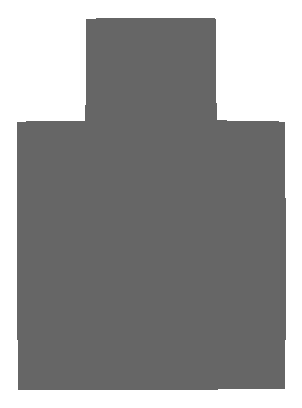
\includegraphics[width=10pt]{figures/face.eps}\hspace{4pt}(\(0\)),
\begingroup\setbox0=\hbox{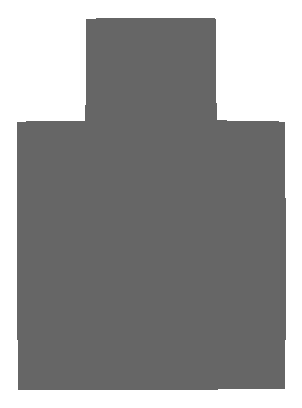
\includegraphics[width=10pt,angle=-90]{figures/face.eps}}\parbox{\wd0}{\box0}\endgroup\hspace{4pt}(\(\frac{\pi}{2}\)),
\begingroup\setbox0=\hbox{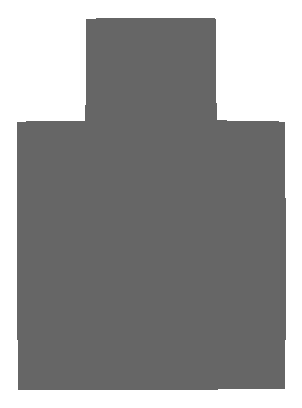
\includegraphics[width=10pt,angle=180]{figures/face.eps}}\parbox{\wd0}{\box0}\endgroup\hspace{4pt}(\(\pi\)) or
\begingroup\setbox0=\hbox{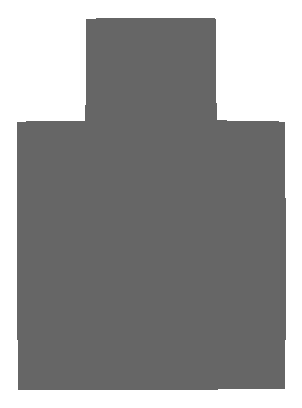
\includegraphics[width=10pt,angle=90]{figures/face.eps}}\parbox{\wd0}{\box0}\endgroup\hspace{4pt}(\(\frac{3\pi}{2}\)), saved as an integer 0, 1, 2, or 3.

For each of the patches, facing left \(\left[-1, 0, 0\right]\), right \(\left[1, 0, 0\right]\), bottom \(\left[0, -1, 0\right]\), top \(\left[0, 1, 0\right]\), back \(\left[0, 0, -1\right]\) and front \(\left[0, 0, 1\right]\) respectively, the default (\(0\)) orientation (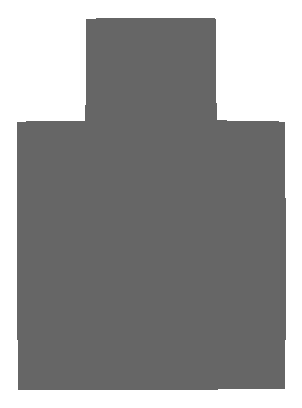
\includegraphics[width=10pt]{figures/face.eps}) corresponds to the vectors \(\left[0, -1, 0\right]\), \(\left[0, 1, 0\right]\), \(\left[0, 0, -1\right]\), \(\left[0, 0, 1\right]\), \(\left[-1, 0, 0\right]\), and \(\left[1, 0, 0\right]\).

A patch can bind to another patch if and only if they have the opposite colour and the same (global) orientation. In Figure~\ref{fig:polycubeRule}, the patch color \(1\) is shown as bright red while the complementary \(-1\) is a darker red colour.  If the patch colour is zero, the patch is shown as empty and will not bind to anything.

The model can be expanded to more complicated colour interaction matrices or changed to pair odd integers with each subsequent integer as in the polyomino model \cite{ahnert2010self,johnston2011evolutionary} described in Section~\ref{sec:polyomino}.

By constraining the input space not to use the back and front patches, while orienting the remaining patches to point towards the front, the output space will instead be 2D polyominoes.

\subsection{String representation}

Polycube rules can be described in a hexadecimal representation, as seen in the Figure~\ref{fig:polycubeRule}.c). Each species is described by 12 hexadecimal digits, two digits per patch. The two hexadecimal digits are then converted into eight binary digits (bits). The first six bits represent the patch colour as a signed integer (allowing for decimal values 0-31); the remaining two encodes one of the four possible patch orientations.

Alternatively, a less compact but more human-readable decimal notation can be used, with each patch written as \texttt{c:o} (where \texttt{c} is the integer colour and \texttt{o} is the integer orientation) and delimited by vertical bars (\texttt{|}). Finally, each species is delimited by underscores (\texttt{\_}). For example, the rule used in Figure~\ref{fig:polycubeRule}, ``\href{https://akodiat.github.io/polycubes?rule=040404040404000000000084}{040404040404\allowbreak000000000084}'', would be written as ``\href{https://akodiat.github.io/polycubes?decRule=1:0|1:0|1:0|1:0|1:0|1:0_|||||-1:0}{1:0|1:0|1:0|1:0|1:0|1:0\_|||||-1:0}''

\subsection{Stochastic self-assembly}
\label{sec:stochastic_assembly}

The stochastic self-assembly of a polycube starts by placing a cube from one of the available species as a seed at the origin. If the assembly mode is \emph{seeded}, it will always use the first species in of rule. If the assembly mode is \emph{unseeded}, the seed species is instead chosen at random. Once a cube has been added to the assembly, all available neighbouring positions are added to a list of possible moves.

Moves are then processed until the list of moves is empty, or the polycube grows beyond a specified size, at which point it is considered \emph{unbounded}. Figure~\ref{fig:UND}.a) shows an example of an unbounded structure tiling the plane using two species.

While the list of moves is not empty, a random move is chosen at each step. The input rule is then randomly searched for a species fitting the move. Cubes can be rotated to fit, and if a fitting species is found, the corresponding cube is added to the assembly. If there is no fit to be found, the move is discarded.
 
The assembly is repeated \(n_{times}\) times (default 100), and the outputs are compared for equality (allowing rotation) in order to determine if the rule is \emph{deterministic}. Figure~\ref{fig:UND}.b) shows a non-deterministic structure, where the blue ``neck'' species can bind to itself. Thus, the output depends on how many cubes from the blue species bind before a green species cube stops the growth. Both species are as likely to bind, so the probability of assembling a neck with \(l\) blue cubes is \(2^{-l}\).

Unbounded or non-deterministic structures are considered \emph{undefined} and are not included in the sampling result. This is in line with the earlier polyomino model and comparable to how unbounded protein complexes or non-deterministically folding proteins are highly deleterious \cite{johnston2021}.


% Unbounded = https://akodiat.github.io/polycubes?rule=05050a08000085858a880000

\begin{figure}
    \centering
    \begin{overpic}[width=\textwidth]{figures/unbounded.png}
        \put(0,630){a)}
        \put(590,630){b)}
    \end{overpic}
    %\centering\includegraphics[width=\textwidth]{figures/unbounded.png}
    \caption{Examples of undefined assemblies.  \textbf{a)} Unbounded assembly that tiles the plane using two species (\href{https://akodiat.github.io/polycubes?rule=05050a08000085858a880000}{05050a080000\allowbreak85858a880000}),  \textbf{b)} An undeterminisic assembly of a ``giraffe duck'' with a neck that can have a different length each time it is assembled (\href{https://akodiat.github.io/polycubes/?assemblyMode=seeded&rule=00000006008b00008600000c000000028c00080c0c000c0c048600000000}{00000006008b\allowbreak00008600000c\allowbreak000000028c00\allowbreak080c0c000c0c\allowbreak048600000000}).}
    \label{fig:UND}
\end{figure}


It could be argued, instead of first picking a random move and then randomly trying all available species to find a fit, that one should pick both a move and a species at random until a fit is found. While this would take a longer time, it would avoid biasing the assembly toward unlikely assembly results, where a move is picked that would otherwise usually be blocked by more likely surrounding cubes. However, since only deterministic and bounded rules are of interest, this would only affect the end result in the cases where the bias is strong enough and \(n_{times}\) is low enough to incorrectly make the rule seem deterministic.


For an illustration of the model, let us return to Figure~\ref{fig:polycubeRule}. The example in the figure is a three-dimensional ``double-cross'' structure created from a rule of size 2. The initial seeding cube belongs to the first species, enabling six additional cubes, all belonging to the second species, to bind at each patch. The patches bind since their colours, \(1\) and\( -1\), are opposites. After all six outer cubes have bound, there are no remaining possible moves, and thus the polycube stops growing. Since the growth stops, this particular polycube is bounded at a size of seven cubes. Furthermore, since the rule gives the same polycube every time it is evaluated, the polycube is deterministic.


%\begin{figure}
%    \centering\includegraphics[align=c,width=0.24\textwidth]{figures/dnaRoboticPolycubes/doubleplus.png}\hfill
%    \centering\includegraphics[align=c,width=0.24\textwidth]{figures/dnaRoboticPolycubes/swimmer.png}\hfill
%    \centering\includegraphics[align=c,width=0.24\textwidth]{figures/dnaRoboticPolycubes/L.png}\hfill
%    \centering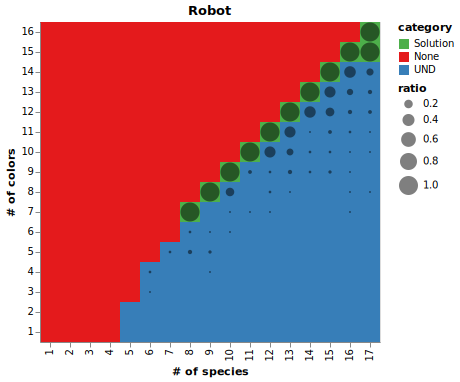
\includegraphics[align=c,width=0.24\textwidth]{figures/dnaRoboticPolycubes/robot.png}
%\caption{Polycube versions of the conceptual DNA Robotics designs. From left to right, the size of the rule required to specify each polyomino is: \href{https://akodiat.github.io/polycubes?hexRule=040890040707840c00000000888a00000000101400000000}{\underline{4}}, \href{https://akodiat.github.io/polycubes?hexRule=0a040b0b080a840e00000000}{\underline{2}}, \href{https://akodiat.github.io/polycubes?hexRule=06000c0b00001284000b080a0090140b00000000188c0000000014980000}{\underline{5}} and \href{https://akodiat.github.io/polycubes?hexRule=0406008800008400240000008c0800000000903400000000980c2f2f10129c1a0000000094000000002214141c000000000028a40000ac3200000000b43000000000}{\underline{11}}. Note how the third polyomino (L-shaped) requires a larger rule than the first (double cross), although it is smaller in size. This is because each cube in the L-shaped nanobot needs to be unique, while the double-cross-shaped first nanobot consists of two identical parts. If we only wished to reproduce the polycube shape, the rulesets could be minimised further.}
%\label{fig:dnaRoboticPolycubes}
%\end{figure}

\subsection{Implementation}

The polycube assembly model is implemented in two versions: one browser-based implementation in JavaScript (\url{https://akodiat.github.io/polycubes}) for outreach activities and accessible visualisation and one C++ implementation for fast rule evaluation. The C++ code also includes a Python binding for simplified analysis. More details on the code can be found in Appendix~\ref{ch:appendix_polycubes}.

%Using the C++ implementation, large sets of random rules have been evaluated, and the resulting polycubes examined and categorised. This has also been repeated for different values of rule size and colour limits.

%See Figure~\ref{fig:rs_vs_ps} for a heat map of the frequency of rules of a certain size creating polycubes of a certain size. Notice how only three different polycube sizes were found for one species. This is understandable when inspecting the first column in Figure~\ref{fig:poly_examples}; using only one species, you cannot create a bounded structure of any other size.

%For larger rule sizes, polycubes can have any form, as shown in Figure~\ref{fig:dnaRoboticPolycubes}, but upon inspection of the larger polycube sizes (and small rule sizes) from Figure~\ref{fig:rs_vs_ps}, the polycubes all seem to be highly symmetrical, as shown in~\ref{fig:poly_examples}.
%I have already implemented a fast version of the code that can generate random rules with a certain max amount of ``colours'' and tile types. The next step is to determine what (deterministic) structures are more common. (Rules creating non-deterministic structures are disregarded, but their percentage of the total is still noted). Plotting the probability of each structure, from a random rule, against a measure of its complexity, do we get a power-law distribution (as in Iain Johnston's polyomino paper)?

\section{Sampling the space of assembly rules}
Trying all inputs in a brute-force approach is unfeasible for most input spaces. For a 3D polycube space with \(\widetilde{K}_s\) species and \(\widetilde{K}_c\) colours, four possible patch orientations, and six patches per species, we get: 
\[
\left\lvert I_{\widetilde{K}_s, \widetilde{K}_c}^{3d}\right\rvert = (4 \times (1+2\widetilde{K}_c))^{6\widetilde{K}_s}
\], where \(I_{\widetilde{K}_s, \widetilde{K}_c}^{3d}\) is the set of all inputs. Even for relatively small values of \(\widetilde{K}_s=3\) species and \(\widetilde{K}_c=2\) colours, we get \(I_{2, 3}^3 \approx 2.62 \times 10^{23}\).

For 2D, it is a bit easier since there are only four patches per species and a fixed patch orientation:

\[
\left\lvert I_{\widetilde{K}_s, \widetilde{K}_c}^{2d}\right\rvert = (1+2\widetilde{K}_c)^{4\widetilde{K}_s}
\]

However, even if the space of possible input rules is too large to explore fully, we can still get an idea of how likely it is for an input rule to map to a particular output shape through uniform sampling. This was done by sampling and assembling a large number of random rules. As described in Section~\ref{sec:stochastic_assembly}, rules growing larger than 100 cubes were discarded as unbounded, while those remaining bounded were re-assembled 100 times to ensure they assembled deterministically. Deterministic and bounded output was then grouped by their shapes, counting the number of times each given shape occurs. For each rule found to produce a given shape, three different complexity measures were calculated:
\begin{description}
    \item[\(\widetilde{K}_s\)] - The number of species used.
    \item[\(\widetilde{K}_c\)] - The number of colours used.
    \item[\(\widetilde{K}_{lz}\)] - The length of the binary rule after Lempel-Ziv compression \cite{lempel-ziv}. 
\end{description}

To more fairly compare them, each rule was simplified before the complexity measure was calculated. This simplification was done by removing all patches without a complementary colour in the same rule, as well as setting the orientation of all empty (zero-coloured) patches to zero. Finally, the colour indices were updated to avoid any gaps in the numbering.

\subsection{Polyomino reference sampling}
\label{sec:refcalc}
% 2D, seeded, 1e9 samples, 16 species, 31 colours
In order to verify the model against earlier polyomino results \cite{johnston2021}, a large reference sampling of the 2D space was performed. Limiting the input space to 16 species and 31 colours (\(I_{16,31}^{2d}\)), one billion (\(10^9\)) random rules were assembled using the seeded assembly mode.

\begin{figure}[ht]
    \centering\includesvg[width=\textwidth]{figures/refcalc/rule_validity.svg}
    \caption{Proportion of valid rules when sampling \(I_{16,31}^{2d}\). From a total of 1,000,000,000 sampled rules, 44,545,570 were found to be valid, while 871,155,425 were  unbounded and 84,299,005 were non-deterministic}
    \label{fig:ref_validity}
\end{figure}

Let us start by looking at the sampled input space. How much of the input maps to valid output? As can be seen in Figure~\ref{fig:ref_validity}, a large number of the sampled rules were either unbounded or not assembling deterministically. The boundary between unbounded and non-deterministic assemblies is not clear, since some input also can be both (but is classified as either one or the other).

Figure~\ref{fig:ref_validity} shows that most of the valid rules assembled into smaller shapes, with over 60 per cent (27 million) being 1-mers (note that the y-axis is logarithmic).

\begin{figure}[ht]
    \centering\includesvg[width=\textwidth]{figures/refcalc/geno_size_distribution.svg}
    \caption{Number of input rules per output size. Distribution of polyomino sizes of \(10^9\) sampled rules in \(I_{16,31}^{2d}\).
    }
    % Ard: The numbering on the x-axis is hard to follow --  I would try to do something like 5, 10, 15 .... Also, there are clear peaks at certain numbers, it is worth mentioning this in the caption or else in the text.
    \label{fig:ref_distr}
\end{figure}

With the input space investigated, we can also check how much of the output space we managed to sample. In Figure~\ref{fig:ref_distr}, the blue bars show how many polyominoes were found of each size, while the red line shows the total number of polyominoes that exist of that size (obtained from the On-line Encyclopedia of Integer Sequences \cite{sloane1995encyclopedia, oeisA000988}). The sampled input space \(I_{16s,31c}^{2d}\) should allow for all 16-mers to be assembled, since there are enough species and colours for fully addressable assemblies (assigning each cube its own species and each connection its own colour). Thus, the blue bars would follow the red line until size 16 if the complete input space was enumerated. Figure~\ref{fig:ref_distr} shows that we find at least the correct order of magnitude up until about 10-mers, after which polyominoes of larger sizes are found in decreasing numbers. Note how some polyomino sizes have a much higher count than their neighbours, indicating a bias for shapes of that size.

\begin{figure}[ht]
    \centering\includesvg[width=\textwidth]{figures/refcalc/pheno_size_distribution.svg}
    \caption{Number of output polyominoes per output size. Count of unique output polyominoes found sampling \(10^9\) input rules in \(I_{16s,31c}^{2d}\). The red line shows the actual number of polyominoes of each size, obtained from OEIS A000988 \cite{sloane1995encyclopedia, oeisA000988}.
    }
    % Ard: Here again, like in 3.4 we see spikes for different sizes -- here not in the number of rules giving polyominoes, but rather in the number of polyominoes found. You need to comment on these two trends, and explain the similarities and differences between them as well.
    \label{fig:ref_distr}
\end{figure}


\subsection{Main samplings}
\label{sec:maincalc}
% use 210924 or 210918?

% 210924: addqueue -n 100 -c "Polycubes long $2 $1D 31c 5t, 2 days" -m 0.5 /users/joakim/repo/polycubes/cpp/polycubes -t 5 -n 1e6 -d $1 -m $2 -r 100 

% 210918: addqueue -n 100 -c "Polycubes long $2 $1D 31c 8t, 2 days" -m 0.5 /users/joakim/repo/polycubes/cpp/polycubes -t 8 -n 1e6 -d $1 -m $2 -r 100

% Better to use 210924 since 3D stochastic is undersampled otherwise
The main sampling was done to compare results between 2D and 3D, as well as the seeded versus unseeded assembly modes. All these samplings were done with \(10^8\) samples each in the \(I_{5s,31c}\) space.

The reason for only using five species per rule is to ensure enough valid output for stochastic 3D, which, as can be seen in Figure~\ref{fig:valid_proportion} is relatively low. 

In general, the seeded assembly mode is expected to generate more valid rules than when the seed is random, as Figure~\ref{fig:valid_proportion} shows. An input rule that depends on the seed can assemble different shapes every time and will be deemed non-deterministic, while the same rule would be considered valid for seeded assembly.  With the third dimension, there are also more orientations and more patches per cube to attach to, leading to the significantly fewer valid 3D rules seen in the figure.

\begin{figure}[ht]
    \centering\includesvg[width=\textwidth]{figures/valid_proportion.svg}
    \caption{Proportion of valid rules when sampling \(I_{5s,31c}\) for seeded and unseeded assembly in both 2D and 3D.}
    \label{fig:valid_proportion}
\end{figure}

Figure~\ref{fig:main_distr} shows the distribution of output sizes for the main samplings. Once again, we can see that the number of shapes found initially follow the same order of magnitude as the total number of existing shapes for each size. Here we can also see even more clearly how shapes of certain sizes show up much more than their neighbours. For example, \(1528\) 36-mers were found in the seeded 3D sampling, while only \(30\) 35-mers and \(58\) 37-mers were found. Such spikes are found for 24-mers, 28-mers, 32-mers, 36-mers, 40-mers, 44-mers, and 48-mers, possibly showing common symmetrical structures growing by four cubes at a time.

% Ard: think we can do better for explanations. It's probably easier to make certain even structures because a single tile can make a dimer, for example.


\begin{figure}[ht]
    \centering\includesvg[width=\textwidth, inkscapelatex=false]{figures/maincalc/distrs.svg}
    \caption{Distribution of output sizes when sampling \(I_{5s,31c}\) for seeded and stochastic in both 2D and 3D. The red line shows the actual number of polyominoes of each size, obtained from OEIS A000988 and A000162 \cite{sloane1995encyclopedia, oeisA000988} respectively.}
    \label{fig:main_distr}
\end{figure}

\section{Symmetry}

For polycube and polyomino symmetry, we care about rotation and reflection symmetry on the lattice. A 2D polyomino has four possible rotations, corresponding to the matrices $\big(\begin{smallmatrix}
    1 & 0 & 0\\
    0 & 1 & 0\\
    0 & 0 & 1\\
\end{smallmatrix}\big)$, $\big(\begin{smallmatrix}
    0 & -1 & 0\\
    1 & 0 & 0\\
    0 & 0 & 1\\
\end{smallmatrix}\big)$, $\big(\begin{smallmatrix}
    -1 & 0 & 0\\
    0 & -1 & 0\\
    0 & 0 & 1\\
\end{smallmatrix}\big)$, and $\big(\begin{smallmatrix}
    0 & 1 & 0\\
    -1 & 0 & 0\\
    0 & 0 & 1\\
\end{smallmatrix}\big)$. The first one is simply the identity matrix and can be ignored. However, if the lattice coordinates remain unchanged after multiplication with any of the others, it means that the polyomino has rotational symmetry. A polyomino also has four possible reflections: one across the x-axis, one across the y-axis, and two along the diagonals. Similarly, a 3D polycube has 24 possible orientations (including identity), as well as reflections around the x-y, x-z, y-z and diagonal planes.

In the simplified context of these lattice shapes, we assign 2D symmetry groups as follows:
\begin{lstlisting}[language=Python]
  if reflsymms == 2:
    group = 'D4'
  elif rotsymms == 3:
    group = 'C4'
  elif reflsymms == 1:
    group = 'D2'
  elif rotsymms == 1:
    group = 'C2'
  elif rotsymms == 0:
    group = 'C1'
  elif reflsymms == 0:
    group = 'D1'
\end{lstlisting}

%For n most common 16-mers, how many of them are symmetrical?

%Freq vs rank coloured by symmetries

\section{Results}

With the sampling details and the analysis methods explained, we will now move on to the main results. Let us start by looking at the different shapes found. Figure~\ref{fig:16-mer_2d_zoo} shows a gallery of the 16-mer polyominoes most commonly found when sampling \(I_{16,31}^{2d}\). Each shape is scaled proportional to the frequency at which it was found, showing that, even within a given size, some shapes are much more common than others.

\begin{figure}[ht]
    \centering
    \includegraphics[width=\textwidth]{figures/16-mers_2d.png}
    \caption{The 50 most common 2-dimensional 16-mers, scaled proportional to their frequency. Found while sampling the \(I_{16,31}^{2d}\) input space.}
    \label{fig:16-mer_2d_zoo}
\end{figure}

Similarly, Figure~\ref{fig:8-mer_3d_zoo} shows a gallery of the 8-mer polycubes found when sampling \(I_{5,31}^{3d}\). Here, the difference in frequency between the shapes was so significant that they instead had to be scaled proportional to the \emph{natural logarithm} of their frequency in order to be visible in the same figure. 
% Ard: Surely the reason for this is that you got a much wider range of structures than for 16mers. -- I'd point out that there are 13,079,255 16mers, but you only find a small number of them -- 

Note how the most common shapes seem to be relatively simple, symmetrical or modular, concepts that will be explored further in coming sections.

\begin{figure}[ht]
    \centering
    \includegraphics[width=\textwidth]{figures/8-mers_3d.jpg}
    \caption{The 50 most common three-dimensional 8-mers, scaled proportional to the natural logarithm of their frequency.}
    \label{fig:8-mer_3d_zoo}
\end{figure}

\subsection{Frequency and rank}
If we plot the frequency of the shapes against their relative rank (with rank 1 being the most frequent, 2 being the second-most frequent, et cetera.), the scaling is quite significant, as seen in Figure~\ref{fig:freq_vs_rank}.

\begin{figure}[ht]
    \centering
    \begin{overpic}[width=\textwidth]{figures/maincalc/freq_vs_rank.png}
        \put(230,300){\large{2D}}
        \put(730,300){\large{3D}}
        \put(10,260){a)}
        \put(480,260){b)}
        \put(950,260){\(\widetilde{K}_{lz}\)}
    \end{overpic}
    \caption{Frequency vs rank for \(10^8\) samples of \(I_{8s,31c}\) in both 2D (a) and 3D (b). Note that the frequency axis is logaritmic. Each point is a unique shape, coloured by its complexity (\(\widetilde{K}_{lz}\)).}
    \label{fig:freq_vs_rank}
\end{figure}

The sharp decrease for the lowest-ranking shapers is a sampling artefact. With a sample size of \(10^8\), a frequency of less than \(10^{-7}\) means that the shape was found fewer than 10 times. Some rare shapes can be found a few times through random chance, giving them a much higher frequency than they would have during a larger sampling.

The sharp decrease among the highest-ranking shapes, however, once again shows how some shapes are much more common than others. Let us see if we can find any features of these shapes that stand out.

\subsection{Frequency and complexity}
% Simple shapes are more frequent.

Let us return to the complexity bias presented in Section~\ref{sec:polyomino_evolve}. Can we show such a trend for the current model as well? Keeping the parameters similar, we start by examining the results of the reference sampling described in Section~\ref{sec:refcalc}. As can be seen in Figure~\ref{fig:freq_vs_compl_refcalc}, there is a log-linear relationship between the probability of finding a rule that assembles into a particular structure and the information needed to specify the structure, as predicted in \cite{dingle2018input, dingle2020generic}.

\begin{figure}[ht]
    \centering
    \includesvg[width=\textwidth, inkscapelatex=false]{figures/refcalc/complexity_vs_freq_16_nc.svg}
    \caption{Frequency vs complexity (\(\widetilde{K}_c\)) of 16-mers found when sampling \(I_{16,31}^{2d}\). Each point represents a unique polyomino shapes, some of which are visualised.}
    \label{fig:freq_vs_compl_refcalc}
\end{figure}

Comparing Figure~\ref{fig:freq_vs_compl_refcalc} with Figure~\ref{fig:polyomino_symmetries}, it is clear that the same simplicity bias is present, reproducing the result from \cite{johnston2021} with the polycube model implementation presented in this thesis. Note how high-frequency low-complexity shapes tend to be more symmetric. The unusually low frequency of the two C2 polyominoes with \(\widetilde{K}_c = 4\) is an example of how the \(\widetilde{K}_c\) measure is an imperfect proxy for Komologrov complexity; both have higher complexity using alternative measures (\(\widetilde{K}_s\)=11 and \(\widetilde{K}_{lz} \approx 211\)). 

Extending our result into three dimensions, as well as using both seeded and unseeded assembly, let us now look at the results from the main sampling, introduced in Section~\ref{sec:maincalc}.

\begin{figure}[ht]
    \centering
    \begin{overpic}[width=0.9\textwidth]{figures/maincalc/freq_vs_compl.png}
        \put(80,-10){Complexity (\(\widetilde{K}_s\))}
        \put(370,-10){Complexity (\(\widetilde{K}_c\))}
        \put(660,-10){Complexity (\(\widetilde{K}_{lz}\))}

        \put(910,870){\small{(unseeded)}}
        \put(910,620){\small{(seeded)}}
        \put(910,370){\small{(unseeded)}}
        \put(910,130){\small{(seeded)}}

        \put(-30,870){a)}
        \put(-30,620){b)}
        \put(-30,370){c)}
        \put(-30,130){d)}

        \put(-100,740){\large{3D}}
        \put(-100,240){\large{2D}}
    \end{overpic}
    \caption{Frequency of shapes found when sampling \(I_{5s,31c}\), versus different measures of their complexity. Each point is a unique polycube (or polyomino) shape, coloured proportional to its size. Each column shows a different complexity measure, as proxies for Komologrov complexity. The left column measures the minimum number of species required to assemble each shape, the middle instead shows the minimum number of colours required, and the right column is the shortest Lempel–Ziv-compressed rule. \textbf{a)} Unseeded assembly in 3D. \textbf{b)} Seeded assembly in 3D. \textbf{c)} Unseeded assembly in 2D. \textbf{d)} Seeded assembly in 2D. Note that the vertical axis (Frequency) is logarithmic.}
    \label{fig:freq_vs_compl}
\end{figure}

As seen in Figure~\ref{fig:freq_vs_compl}, the simplicity bias is still present for 3D polycubes, even using alternative measures of the complexity. The measures provide different resolutions, but all still show the frequency of a shape bounded by its complexity. 

One apparent break from the trend shown is the mostly constant \(\widetilde{K}_s\) values for unseeded samplings (Figure~\ref{fig:freq_vs_compl}.a) and~\ref{fig:freq_vs_compl}.b)); almost all the output shapes use the maximum number of species. This can be explained as a consequence of the determinism check. A seeded rule can afford to have a few non-binding species that are simplified away and not counted, as long as none of them are the seed. But with unseeded assembly, any species can be the seed; so such a rule would be deemed non-deterministic and not included. Thus, for the unseeded results, we have to rely on the other two complexity measures.


\subsection{Modularity}

Besides symmetry and complexity, we can also look at how the modularity of a shape can limit its frequency. We use a simple \emph{modularity index}, defined as the polycube size divided by the number of needed species (\(\widetilde{K}_s\)). Basically, a modular shape is one where modules are reused many times. For the reasons detailed above, it only makes sense to look at the modularity of seeded assemblies since \(\widetilde{K}_s\) is otherwise primarily constant.

\begin{figure}[ht]
    \centering
    \begin{overpic}[width=\textwidth]{figures/modularity/modularity_6-10.eps}
    \end{overpic}
    \caption{Frequency vs modularity for a selection of sizes. The top row shows 2D polyominoes, while the bottom row shows the 3D polycubes. From 1e8 samples of \(I_{8s,31c}\).}
    \label{fig:freq_vs_modularity}
\end{figure}

Figure~\ref{fig:freq_vs_modularity} shows how the modularity correlates with the frequency for a selection of sizes in both two and three dimensions. For a fixed size, the modularity index is really only a scaled inverse of the \(\widetilde{K}_s\) complexity, but it is still helpful to see how modular shapes have a significantly higher frequency.

We have now shown how simple designs can be found through random sampling, but how would one go about designing a rule that assembles a specific shape? And does it matter if the rule is simple or not? That will be covered in the coming chapter.

% Modularity and robustness https://www.tandfonline.com/doi/full/10.1080/09544828.2019.1686469




%\section{Robustness}

